\chapter{The ARIO model in the literature of indirect economic costs}
\label{sec:descr-ario-indir}

\section{Introduction}

Here we present a quasi-exhaustive review of the literature associated
with the ARIO model.

In their comprehensive review on methodologies for assessing the economic
impacts of natural disasters, \textcite{botzen-2019-econom-impac}
introduce the ARIO model as an attempt to overcome the limitations inherent in
conventional Input-Output (IO) models. Likewise, the work by
\textcite{galbusera-2018-input-output}, which
focuses on IO-based models, highlights the ``additional features''
incorporated into the ARIO model to address the same limitations.

In~\textcite{coronese-2022-econom-impac}, authors advocate for complexity methods and
Agent-Based Models (ABMs) to study indirect impacts from disasters. In their
extensive review of the literature, they position ARIO both as an IO model and a
``renowned'' hybrid model.

These three contributions all underscore the following notable aspects of the ARIO model:
\begin{itemize}
\item It operates as a dynamic model (computing the state of the economy over multiple
steps after the shock rather than only statically determining the new
equilibrium in the aftermath).
\item It integrates various adaptation processes (such as overproduction, (some) suppliers substitution, and resiliency measures).
\item It considers shocks both on production and demand.
\item It employs a rationing scheme to resolve the disequilibrium between
production and demand.
\end{itemize}

\Textcite{hallegatte-2013-model-role} extends the version presented
in~\textcite{hallegatte-2008-adapt-region} by introducing
inventories of inputs. This new aspect enables a better representation of the filling, depletion and scarcity of
different inputs in the model, and the possible consequent supply-chain
disruptions.

As such, the ARIO model is considered as a suitable middle-ground between basic
IO models and advanced ABMs. It requires limited input data and parameter
configuration compared to more complex models while allowing for emerging
dynamics and more advanced evaluations of indirect economic impacts from disasters.

In the following section, we review the literature associated with the ARIO
model. We focus on articles that either use, extend or assess the ARIO model and also
include several publication presenting closely related models. Next, in the last section of
this chapter, we provide an in-depth and commented description of our version of
the model and its Python implementation
[\href{https://spjuhel.github.io/BoARIO/}{BoARIO}].

\section{Literature review}
\label{sec:ario-literature}

\begin{figure}[h!]
  \centering
  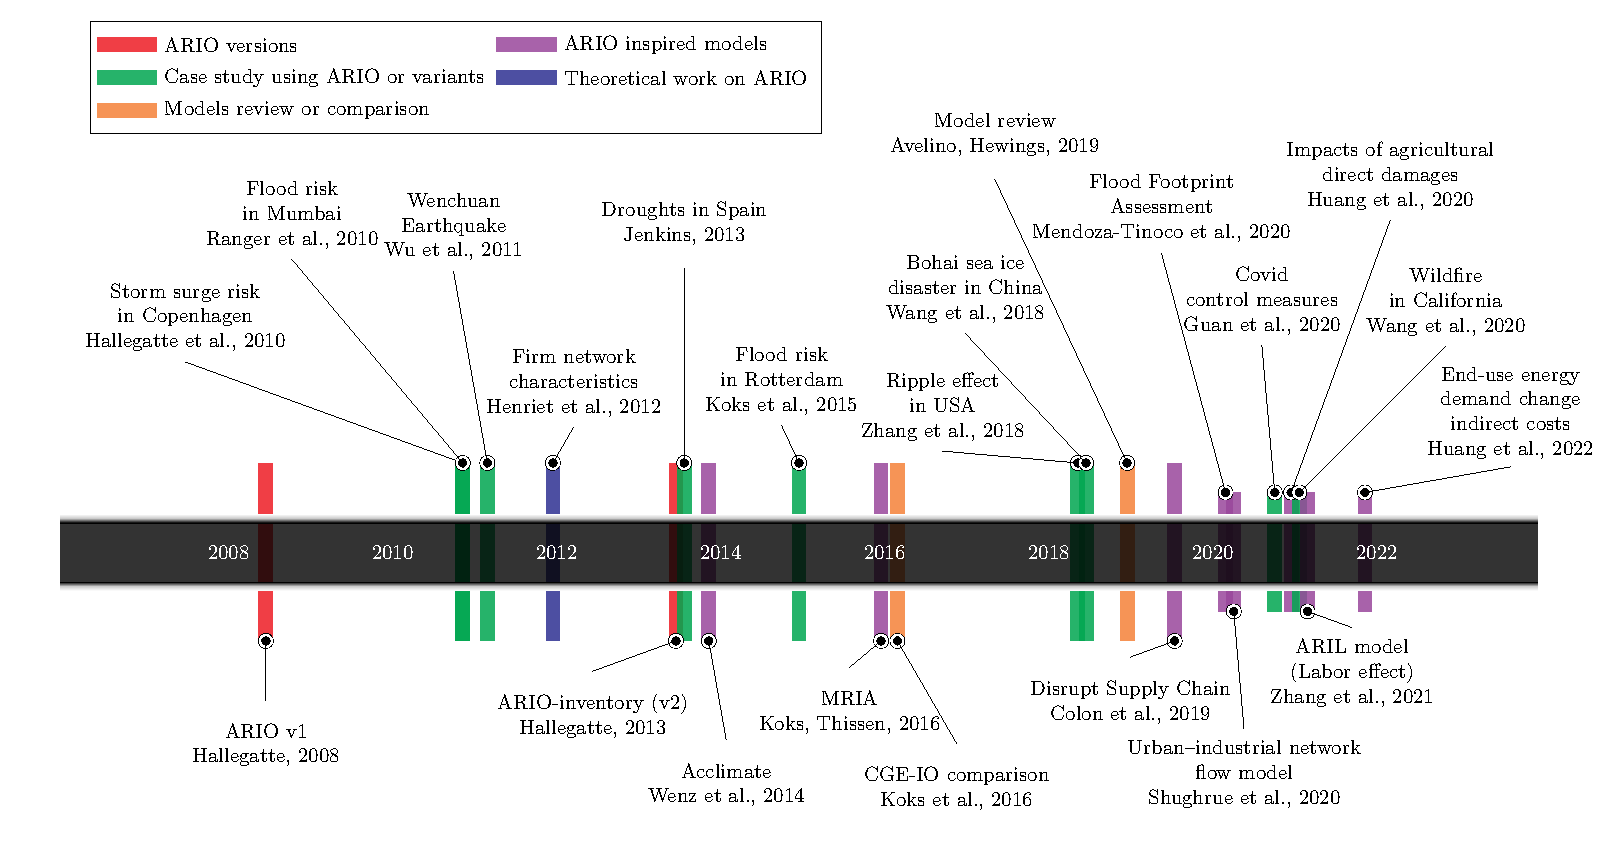
\includegraphics[width=\textwidth]{ario-chronology.pdf}
  \caption{Literature related to the ARIO model\label{fig:ario_chronology}}
\end{figure}

\subsection{2008-2012 -- Seminal works with the ARIO model}
The seminal work of~\textcite{hallegatte-2008-adapt-region}
serves as the cornerstone for the ARIO model, introducing it as an innovative
Input-Output (IO) based framework capable of accounting for both forward and
backward indirect costs, alongside adaptive behaviors manifested through
alterations in imports. The article showcases the model using the case-study of
the economic impacts on the state of Louisiana from Hurricane Katrina.
To establish regional tables for Louisiana,
the author employs national IO
tables provided by the U.S. Bureau of Economic Analysis. These national IOTs are
downscaled to the Louisiana level, assuming proportionality between value added,
total output, wages, and intermediate consumption per industry and their
respective gross products at the state level. Export are assumed to represent
half of local production except for the mining sector,
where 75\% of the gross output is exported. The allocation of intermediate
demand, whether sourced locally or imported, mirrors the production ratio.

Direct damages attributed to Katrina are estimated at~\textdollar107 billion and
distributed across government, housing and industrial sectors based on an
evaluation by the Committee on the Budget U.S. House of Representatives.
Moreover, 75\% of those damages generate an additional demand towards the
Construction sector, while the remaining 25\% are directed toward the
manufacturing sector. With these values, the author
finds an amplification ratio of 1.39 (i.e., total economic losses represent
139\% of the direct losses). The author also note:
\begin{itemize}
\item The absence of forward propagation of the shock (production is never limited
by an input shortage).
\item Indirect impacts are tied to substantial backward propagation in the model.
\item Indirect losses increase non-linearly with direct losses.
\end{itemize}

In~\textcite{hallegatte-2010-asses-climat}, authors conducted an
assessment of storm surge risk in Copenhagen, with the help of the ARIO model to
evaluate the indirect costs part of this risk. Their evaluation encompasses expected change in storm
surges risk in the context of sea level rise and Copenhagen's exposure to coastal
flooding. They derive possible direct losses as a function of flood
depth using vulnerability curves tailored for multiple return periods and varying levels of sea
level rise. The direct losses estimates then serve as an input for the ARIO
model. The model relies on economic data obtained from StatBank Denmark and on the Danish
national IO table, downscaled to Copenhagen using a methodology akin to that
employed in~\textcite{hallegatte-2008-adapt-region}. The outcomes of
this study indicate that Copenhagen is well-protected against present and future
storm surges. Nevertheless, the authors underscore certain limitations that
could lead to an underestimation of total losses. These limitations
include the coarse estimation of infrastructure vulnerability and the
methodology applied to assess direct losses, which notably omits the influence
of water velocity on damages.

\textcite{ranger-2010-asses-poten} undertake a similar study to
assess potential impacts of floods in Mumbai in the context of climate change.
They use their evaluation of the direct impacts of the July 2005 flood in Mumbai
as a shock for the ARIO model.  Several modifications to the ARIO model are
introduced in this study, including a shorter reconstruction duration (3 months)
and an adjusted rationing scheme that prioritizes local demand. This entails
serving intermediate consumption first, distributed proportionally among
industries, followed by addressing reconstruction needs and final demand, and
ultimately fulfilling export requirements. Unlike previous studies, this
version of the model no longer assumes that direct losses are entirely
covered by insurance, thereby significantly impacting household budget dynamics.
The authors evaluate how two distinct adaptation policies can help reduce indirect
losses: enhancing the flexibility of the construction sector's capacity and
increasing insurance coverage. Their findings indicate that expediting the
response of the construction sector to reconstruction demand can reduce indirect losses
by a factor of up to 4, while increasing insurance coverage to 100\% has the
potential to halve indirect losses.

\textcite{wu-2011-region-indir} evaluates the
indirect costs of the Wenchuan Earthquake, focusing on the impact in the Sichuan
Province. The study relies on local IO tables from the Sichuan Provincial Bureau of
Statistics coupled with estimates of direct losses per sector, obtained
from the National Commission of Disaster Reduction and the Ministry of Science
and Technology of China. The authors find that indirect losses amount to 40\% of the
direct losses and that the reconstruction period predicted by the model spans
over 8 years. The authors draw attention on how changes in the demography as
well as in the growing  economy of China are not accounted in their analysis and
how that would probably affect the reconstruction process.

In a more theoretical work, \textcite{henriet-2012-firm-networ}
extend the ARIO model towards a more agent-based approach. This is done through
a disaggregation of the sectors into production units (PU) representing firms
instead of whole economic branches. The network connecting these PUs
is randomly generated with a set of constraints such as the number of PUs per
sector or the number of suppliers per PU. The goal of this innovative framework
it to provide insights into the economic robustness of firms network.
The authors demonstrate how this theoretical disaggregation aggravates indirect
losses following a shock compared to classical IO tables. Furthermore, they also
show how bigger inventories increase the time during which PU can maintain
production after the shock thereby reducing the likelihood of shortages and
mitigating indirect losses. Another key observation of the study is the
elucidation of how the heterogeneity of losses influences indirect losses.
Specifically, when a shock is concentrated on a few PUs, the total losses are
markedly higher compared to a scenario where the same shock is distributed among
a larger number of PUs. This finding implies that locally concentrated disasters
have the potential to exert more profound economic impacts than more evenly
distributed disasters.

In the study conducted in~\textcite{jenkins-2013-indir-econom}, the ARIO
model serves as the main tool to investigate indirect losses caused by droughts
under future climate change in Spain. The author projected estimates of drought
related direct losses per sector, for different climate
scenarios. Losses per sector are distributed according to their water-use. A
notable assumption in this research is the absence of additional demand stemming
from reconstruction efforts. This is based on the understanding that
droughts, unlike other disasters, do not involve the destruction of productive
capital but instead result in temporary losses in production capacity, which
can be reinstated without necessitating extensive reconstruction efforts.
Results suggest that total losses from drought could be increase by 30
(short-term droughts) to 60\% (long-term ones) when considering indirect losses.
This study also finds a non-linear increasing relationship of indirect losses
with the intensity of the drought.

\subsection{2013-2016 -- ARIO-inventories, MRIA and Acclimate}

In~\textcite{hallegatte-2013-model-role}, the author enhances and
updates the ARIO model presented in his previous
work~\citeyear{hallegatte-2008-adapt-region}, with another
evaluation of the indirect losses in Louisiana following Katrina, now with a
more elaborated version of the ARIO model alongside more precise economic and
direct loss data. The most prominent improvement brought to the ARIO model in
this article is the explicit representation of input inventories. This addition
significantly improves the model's ability to capture bottlenecks and further
positions this model as a ``middle-ground solution''
between IO and CGE models in the short-term analysis of disaster impacts. In
his study, \textcite{hallegatte-2013-model-role} emphasizes
how the key contribution of their case study is not the indirect cost
quantitative estimation, rather than the identification of two distinct dynamics
following the disaster. A first period which witnesses the majority of the
indirect losses, primarily driven by forward propagation of ripple effects
(through production bottlenecks\footnote{Which contrasts with results
  in~\textcite{hallegatte-2008-adapt-region}}). Subsequently, a
second period ensues, dominated by the reconstruction process, where
bottlenecks are not observed and indirect losses are lower. The paper also
evaluates the sensitivity of the model to its different parameters and finds the
heterogeneity parameter (see~\cref{sec:invent-constr} for details on this
parameter) to play a key role in the results.

In their study,
\textcite{koks-2014-integ-direc} investigate the indirect
costs associated with flood events in Rotterdam, employing the version of
ARIO introduced in~\textcite{hallegatte-2013-model-role}.
The author bring a notable enhancement to the model by incorporating a Cobb-Douglas
production function, applied to capital and labor, to estimate the inoperability
of affected sectors due to the reduction of both these variables. A significant aspect of their analysis is the global sensitivity assessment
of the model they conduct. The study uses a Monte Carlo approach to identify
parameters with significant influence on the outputs. Their findings reveal that
the influence of parameters varies across different levels of flood severity.
For rarer and more destructive floods, changes in the internal heterogeneity of the
sectors (commonly denoted by $\psi$ in the ARIO model literature) exhibit a
greater influence than the speed of reconstruction.
Conversely, for less destructive floods, the speed of reconstruction plays a
more prominent role. The study also uncovers threshold effects in flood impact, particularly
regarding flood duration. The analysis indicates that indirect damages exhibit a
predominantly linear relationship with flood duration, up to a certain threshold
(280 days in their case). Beyond this point, a notable increase in indirect losses
is observed, which shows a distinct recovery dynamic in this case.

In~\textcite{koks-2016-multir-impac}, the authors introduce the
\acrfull{MRIA} model, a ``recursive dynamic multi-regional supply-use model''
designed for the analysis of natural disasters impacts on the economy. Similarly to
the ARIO model, the MRIA model finds its theoretical basis in IO modeling, but
as a key additional characteristic, it makes use of linear programming (LP)
techniques to improve on traditional IO models. These LP techniques are used to
find optimal solutions to balance production and demand while accounting for a
set of constraints, for instance on production capacity and reconstruction
demand. Another distinctive feature of the MRIA model, in contrast to the
version of the ARIO model presented in~\textcite{hallegatte-2013-model-role}, is its capacity for regional
substitution, effectively mitigating indirect losses. The article showcases the
model on three different flood scenarios in Rotterdam,
using a MRIOT of 256 European regions a the NUTS2 level, as an economic input.
Their results show that Regions adjacent to the affected area experience
increased demand for reconstruction, leading to gains, while regions further
away or lacking a direct export link incur relatively minor losses. The study
also highlight that the relationship between direct and indirect impacts
they find contrasts with the results found
in~\textcite{koks-2014-integ-direc, hallegatte-2013-model-role}. These two previous studies found
indirect losses to become higher than direct ones after a certain threshold, while
in this one, indirect impacts remain lower than direct ones even for a 1 in
10000 flood. This difference is attributed to the regional substitution
mechanism in the MRIA model. The authors position their model as an even closer
to CGE approaches (such as~\textcite{carrera-2015-asses-direc}) compared to the
ARIO model.

In a comparative analysis, \textcite{koks-2016-region-disas} assess
three hybrid models: the ARIO model, the Multi-Regional Input-Output and Asset
(MRIA) model \parencite{koks-2016-multir-impac} discussed
previously, and the Interregional Environment-Economy Simulation (IEES) model, a
sub-national Computable General Equilibrium (CGE) model based on the Global
Trade Analysis Project (GTAP) \parencite{hertel-1997-global, narayanan-2008-global-trade}. The flood scenario chosen for this comparison
unfolds in the Po River basin in Italy. The authors hypothesize that the duration and shape of the recovery
path has a significant influence on total losses. To test this hypotheses, they
compare three different recovery curves (concave, convex and linear). The study
finds that estimated total economic losses vary significantly between the three
models. Specifically, the ARIO model exhibits higher losses compared to the MRIA and IEES
models. The regional distribution of losses across
Italy also differs among the models: while total economic impact is negative for
all models in the affected region, the impacts are positive in unaffected
regions for the IEES and the MRIA model and negative for the ARIO model.
Additionally, the study identifies a correlation between the speed of
recovery and the magnitude of losses with quicker recovery being associated with lower
losses.


\Textcite{bierkandt-2014-acclim-model, otto-2017-model-loss} introduce and expand upon the
Acclimate model, a numerical dynamic agent-based model that shares several
similarities with the ARIO model: the underlying economic network is also based on
an MRIOT which dictates how production agents initially trade among themselves and with
consumption agents. The model also uses a Leontief production function (inputs are considered perfectly complementary). Direct Damages are translated into losses
of production capacity (either \emph{via} exogenously imposed losses or productive
capital destruction) and changes in final demand. Production agents adjust or
extend their output as the demand changes, and can warehouse inputs in
storage to buffer out failures in delivery. The Acclimate model also brings
several additional mechanisms and improved aspects compared to the ARIO model:
first MRIOTs are disaggregated to the administrative region level, in order to
better match the actual size of disaster
areas \parencite{wenz-2014-region-sector}, second the authors
add a transportation layer which accounts for the transit time of goods between
regions. In~\textcite{otto-2017-model-loss} the authors further
extend the model such that agents use prices as an ``organisation
mechanism'' where firms make decisions about their production levels and
suppliers based on profit maximization. This extension enhances the realism of
the model by introducing a market-oriented decision-making process, reflecting
the economic dynamics more accurately.

\subsection{2018-Today -- New variants and rise of ABMs}

In their article, \textcite{zhang-2018-analy-econom} introduce
the International Ripple Effect Input-Output (IREIO) model to evaluate how
climate change impacts in the USA lead to economic repercussions in other
regions. The IREIO model is based upon the ARIO model, which is extended to work
at the multi-regional scope with the help of an MRIOT. Another enhancement
adapts the ARIO model for the purpose of evaluating climate change impact on
working hours. The primary focus of the study is on indirect costs stemming from
climate change impacts on agricultural yields, labor supply, and energy demand
within the USA. The findings reveal that indirect costs in the rest of the world
can reach up to a third of the direct costs incurred in the USA, representing
slightly below 1\% of the USA's Gross Domestic Product (GDP).
Authors assess the general sensitivity of the model to a range of values for its
parameters of their model but do not assess in detail how each parameters influence
their results. Furthermore, it is worth noting that this study uses
an ARIO-based model to evaluate how gradual changes lead to indirect costs,
rather than focusing on the repercussions of sudden shocks, which may stretches
the ARIO model beyond its intended scope.

\textcite{wang-2018-quant-spatial} develops the Inter-Regional
Input-Output (IRIO) model, also based on the ARIO model \parencite[version
from][]{hallegatte-2008-adapt-region}, to replicate the indirect
economic losses resulting from the Bohai Sea ice disaster event. One of the main
focus of the study is the spatial heterogeneity of
affected economic structures, which authors achieve by adapting the ARIO model
to a MRIOT framework, that distinguishes 31 provinces in China. Their findings
reveal that while a significant portion of the indirect losses in
China occurs in the affected areas (representing 61\% of total indirect losses),
regions not directly impacted also experience indirect losses. Provinces adjacent to
the directly affected ones are among the most indirectly affected, but the study
also identifies remote provinces that exhibit noticeable impacts. Interestingly, more
developed provinces incur higher indirect costs than less developed ones.
Overall, authors highlight how accounting for the heterogeneity of the economic
structure heavily influence the results.

\Textcite{colon-2020-critic-analy, colon-2019-trans-suppl} draws on
the work from~\textcite{hallegatte-2008-adapt-region, henriet-2012-firm-networ, hallegatte-2013-model-role} to introduce the Disrupt Supply
Chain model.  This agent-based model incorporates an explicit transportation
network and is designed to assess the economic consequences of disruptions in
transport infrastructure. Key components of the model include mapping production
and consumption agents (representative firms and households) to geographical
``Origin-Destination (OD) nodes'',
constructed from transportation infrastructure, population data, and GDP.
Supply-chains flows between agents are established from IO tables and are associated
with paths in the physical transportation network. The model also incorporates a
distance based transportation cost. Firms within the model hold inventories of
inputs similar to those in the ARIO model. One key feature of the model comes
with the fact that it enables the assessment of the economic consequence of a
transport infrastructure disruption, and the rerouting or shortages that may
follow. As a disruption happens, inputs prices rise (from the rerouting costs or
the scarcity) and firms adjust theirs selling price to preserve their profit.
The authors illustrate the model on the Tanzanian road network, by assessing its
criticality, i.e., assessing which assets cause the highest
impacts when disrupted. They find this criticality to differ from sector to
sector (e.g., critical roads are not the same for food security and national
trade) and also find that indirect economic losses are non-linear relative to the
duration of transport disruption. Furthermore, this model highlights how policy
measures to enhance supply chains resilience can act on several other aspects
than improving the transport infrastructure, such as sourcing decisions and
inventory management.

In~\textcite{avelino-2019-chall-estim}, the authors review multiple
IO-based approaches used to estimate the impact of disasters and their
limitations and present a model framework (named Generalized Dynamic
Input-Output or GDIO) to extend those approaches, building on the ``fragmented''
contributions of the different models reviewed, ``especially those contained in
the ARIO model''. The authors notably acknowledge how the ARIO model includes many of the
contribution of previous literature on dynamic/hybrid IO modeling.
However they also underscore the absence of a real production scheduling
mechanism, the oversight of seasonality of
production \parencite{avelino-2017-disag-input}
(e.g. for the agriculture sector), and a lack of consideration for demographic
dynamics post-event. To illustrate the application of the GDIO framework, the
authors provide a
simple example in an abstract mono-regional, three-sector economy. The
comparison with other dynamic IO models, including the ARIO model, reveals that
GDIO presents a more complex response, characterized by non-monotonic and
non-smooth recovery dynamics. This complexity is attributed to the explicit consideration
of the labor market and the use of the Sequential Inter-industry Model
framework, which does not assume simultaneous production across sectors.
It is noteworthy that, while the authors emphasize the unique features of GDIO,
they acknowledge that the ARIO model produces results closest to their own in
the comparative analysis.  To our knowledge no ``real natural disaster''
application of this model exists in the literature.

\Textcite{mendoza-tinoco-2020-flood-footp-asses, mendoza-tinoco-2017-flood-footp} couples the ARIO model~\parencite[version
from][]{hallegatte-2008-adapt-region} to the
Basic Dynamic Inequality (BDI)
model~\parencite{li-2013-model-imbal}. The BDI model allows to
evaluate production capacity losses from natural disasters impacts on labor force and
residential assets. This tandem of model results in a flood footprint model
applied to both mono-regional~\textcite{mendoza-tinoco-2017-flood-footp} and
multi-regional~\textcite{mendoza-tinoco-2020-flood-footp-asses} settings.
In~\textcite{mendoza-tinoco-2020-flood-footp-asses} the authors also incorporate a
``\emph{capital matrix}'' detailing the input structure of productive
capital stock per region and sector, and ground the reconstruction demand on
this matrix. The study also considers change in final demand following the disaster,
where final consumers reduce their demand for ``non-basic products'' in the
immediate aftermath and progressively increase it back as the economy recovers.
The model is applied to the 2009 European floods and the authors find
that indirect losses represent 65\% of the total losses in this setting. Notably they
observe that industries at the end of the supply chain suffer bear the major
share of indirect losses and that large and developed economies are more susceptible
to face significant indirect losses than less-developed ones, due to their higher
capital intensity and ``strong[er] interindustrial links''.

\Textcite{shughrue-2020-global-spread, shughrue-2018-system-vulner} contribute to the field by
introducing the UrbaN Industrial connectivity Risk Network (UNICORN), a global
urban-industrial network dataset. In contrast to conventional multi-regional
frameworks, their model describes the global economy as a network of cities
instead of economic regions. The proposed network is made up of ``1686 cities with more
than 300000 inhabitants'' and details the production flows in-between them.
Drawing inspiration from~\textcite{wenz-2016-enhan-econom,
  hallegatte-2013-model-role}, the authors introduce a model
based on this network, which incorporates the main elements of the ARIO model,
such as the reconstruction process, inventories of inputs and overproduction,
but also ones from the Acclimate model, such as profit optimization and
suppliers adjustments. The application of this model focuses on assessing the
propagation of indirect losses triggered by cyclones. Noteworthy findings
include the identification of North America and East Asia as regions generating
the highest indirect losses, while Europe benefits from shifts in supply
dynamics. The study also observes the rapid propagation of detrimental indirect
impacts, manifesting through swift increases in prices. Interestingly,
beneficial impacts are delayed, occurring 6 to 24 months after a direct loss.
Much like the rest of the literature, the study highlights the non-linear
relationship between direct and indirect impacts, showcasing the presence of a
threshold beyond which indirect impacts become more severe.

\Textcite{guan-2020-global-suppl} enhance the ARIO
model \parencite[version from][]{hallegatte-2013-model-role}, by
introducing more dynamic choices of suppliers (which we describe in detail
in~\cref{par:orders_sh}) and adapting it to a multi-regional framework. This
upgraded model is then applied to simulate various COVID-19 containment
scenarios, incorporating factors such as labor availability and transportation
restrictions, with the aim of assessing their potential impact on the global
economy. The study reveals that supply-chain losses are contingent on the number
of countries implementing restrictions. Furthermore, it suggests that longer
containment periods with disease eradication result in smaller losses, while
earlier, stricter, and shorter lockdowns prove effective in minimizing overall
losses.

\Textcite{huang-2020-asses-econom} uses the ARIO model \parencite[version
from][]{hallegatte-2008-adapt-region} to assess indirect losses
stemming from direct economic impacts of climate change on the agriculture sector in
China. The study uses a local IOT specific to China in 2012 and uses crop yield
data under future climate change from~\textcite{liu-2020-centr-trend} to infer
direct economic losses in the agriculture sector. Results highlight that
indirect losses are substantial as they amount to 4.24 to 5.25 times the direct
losses. Note that this seemingly high estimation may be tied to the use of the
original version of ARIO which enabled limited adaptation mechanisms.
The manufacturing sector emerges as the most affected (25\% of the indirect
losses) followed by the agriculture and construction sectors.

\Textcite{wang-2020-econom-footp} conduct a comprehensive assessment
of the economic footprint of the 2018 California wildfires. In particular, the
study employs a Multi-Regional Disaster Footprint (MRDF) model, presented as an
extension of the ARIO model introduced
by~\textcite{hallegatte-2008-adapt-region}. This adaptation
transforms ARIO into a multi-regional framework. Utilizing linear programming
techniques, akin to the approach
in~\textcite{koks-2016-multir-impac}, the model optimizes
the
output of each sector, considering constraints related to technology (production
functions), remaining productive capital, working time, transportation,
intermediate demand, and total demand. Their results indicate that
indirect losses constitute a important share of the total losses, representing
59\% of them and amounting to~\textdollar88.6 billions. Additionally, noteworthy
observations emerge, revealing that these indirect losses often extend their
impact to industries not directly reached by the wildfires.

\Textcite{zhang-2021-analy-impac} introduce the Adaptive
Regional Input-Output With Inventory and Labor (ARIL) model, constructed from
the ARIO model~\parencite[version
from][]{hallegatte-2013-model-role}. This version mainly adds the
consideration for short-term shortage of labor supply in the aftermath of a
disaster. The authors use this improved version to study the 2016 extreme flood
in Wuhan City in China. They focus on the concept of resilience, which they
assess based on the shape of the recovery path of change in value added. They
evaluate the effect of seven scenarios of rescue funds and find that these funds
can mitigate or even prevent some of the adverse indirect impacts caused by a
disaster.

In their study, \textcite{huang-2022-estim-poten} extend the ARIO model by
incorporating Energy-IO tables, enabling the model to consider the demand for
end-use energy. This extension is employed to evaluate the economic implications
of climate change restrictions on ``conventional'' energy use in China. The
research compares various scenarios of restriction and examines their impact on
China's GDP. Their findings reveal that achieving a carbon emission peak in
China before 2030 requires restrictions on total energy consumption, resulting
in significant GDP indirect losses, approximately 15\%,
with the industrial sector experiencing the most pronounced impact due to its
high energy consumption. It is crucial to highlight that, unlike the rest of the
literature, this article uses the ARIO model for long-term assessments,
focusing on the absence of a specific input (energy use), and the results may be
perceived as relatively pessimistic compared to other modeling methodologies
such as CGE or Integrated Assessment Models (IAM).

\section{Code availability of ARIO implementations}

\notebox{ Few articles give access to the model implementation used. We had
access to a Matlab version of ARIO from S. Hallegatte but to our knowledge no
online repository exists. Otherwise we found the following implementation
online:

  \begin{itemize}
  \item A python implementation of MRIA is available on the personal GitHub
repository of E. Koks (\url{https://github.com/ElcoK/MRIA}) though we did not
find a mention of it in its seminal
paper \parencite{koks-2016-multir-impac}.
\item C. Colon mentions his repository for a python implementation of Disrupt
Supply Chain in~\textcite{colon-2020-critic-analy}.
\item A C++ implementation of Acclimate is available here
\url{https://github.com/acclimate/acclimate}.
\item A Matlab implementation of C. Shughrue's model developed
in~\textcite{shughrue-2020-global-spread, shughrue-2018-system-vulner} is available at
\url{https://github.com/chrisshughrue/GlobalUrbanCycloneImpactSimulation}
\item The models used
in~\textcite{wang-2020-econom-footp, guan-2020-global-suppl} are both available at
\url{https://github.com/DaopingW/}
\end{itemize}
We note here that most articles we reviewed which use the ARIO
model do not provide an explicit implementation of the model they use, and as
several version and setups of the model exist, it makes it difficult to compare
these different studies, as well as reproducing them. This is one of the reason
we developed a versatile and modular version of ARIO in python.}


In conclusion, this comprehensive literature review has shown the
versatility and significance of the ARIO model in studying the propagation of
economic shocks: from the aftermath of natural disasters to the complex dynamics of
climate change induced impacts and global disruptions such as the COVID-19
pandemic. Initially
introduced by~\textcite{hallegatte-2008-adapt-region}, the ARIO
model has emerged as an adaptable tool, integrating input-output
structures, dynamic features, and adaptive behaviors to bring a more nuanced
approach than traditional IO models. The examined studies have showcased its
applicability across various contexts, demonstrating its utility in regional,
sector-specific, and global supply chain analyses. Evolving over time, as
demonstrated by~\textcite{hallegatte-2013-model-role}
and~\textcite{guan-2020-global-suppl}, the model has
incorporated additional elements such as inventories, labor considerations, and
global economic connections. This review however highlights some research gaps
on the robustness of the ARIO model. Particularly, we observe a certain scarcity
of studies assessing the sensitivity of the model when employing multi-regional
input-output tables (MRIOTs) and extending the model to encompass multi-regional
trade. Furthermore, we observe the absence of a
comprehensive analysis evaluating the impact of the choice of economic data,
specifically the choice of the MRIOTs describing the initial state of the
economy in a multi-regional framework. We also note that the specific setup
(parameters, version used) of the ARIO model in the different studies reviewed
is not always explicit, while several sensitivity analysis at the local
framework have shown the model to have a high sensitivity to its parameters.
These observations lay the groundwork for the sensitivity analysis undertaken in
the subsequent chapter, aiming to address these gaps and enhance our
understanding of the ARIO model's applicability across diverse economic scales
and research questions.

%%% Local Variables:
%%% mode: LaTeX
%%% TeX-master: "main"
%%% End:
